\documentclass[11pt, oneside]{article} 
\usepackage{geometry}
\geometry{letterpaper} 
\usepackage{graphicx}
	
\usepackage{amssymb}
\usepackage{amsmath}
\usepackage{parskip}
\usepackage{color}
\usepackage{hyperref}

\graphicspath{{/Users/telliott_admin/Dropbox/Tex/png/}}
% \begin{center} 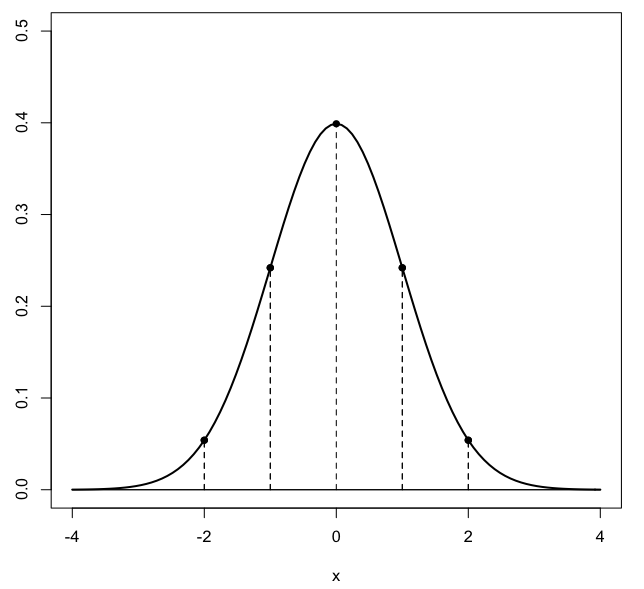
\includegraphics [scale=0.4] {gauss3.png} \end{center}

\title{Real numbers 2}
\date{}

\begin{document}
\maketitle
\Large

\subsection*{number line}
A simple tool to visualize all of the real numbers is the familiar number line.  Here is the number line in terms of $\mathbb{N}$, but obviously we could also draw one for $\mathbb{Z}$ or $\mathbb{Q}$.

We explore the application of the number line to $\mathbb{R}$ as we proceed.
\begin{center} 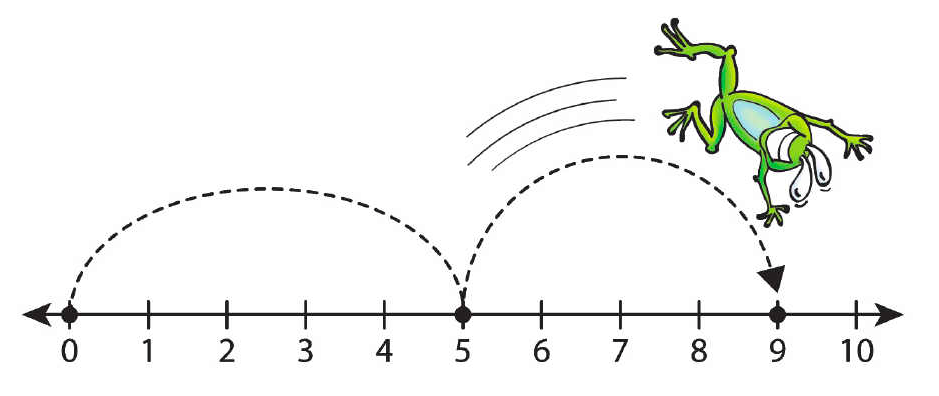
\includegraphics [scale=0.4] {number_line.png} \end{center}

We might simply assume that to every point on the number line there corresponds a rational or irrational number, and that this total collection obeys the same laws of arithmetic as the rational numbers do.

As mentioned above, the need for the real numbers is indicated by empty "holes" in the number line corresponding to the irrational numbers like $\sqrt{2}$.

A problem that arises is how to specify an irrational number non-geometrically and other than as the solution to an equation such as $r^2 = 2$.  In all cases we write particular real numbers as \emph{approximations}.  For example, the square root of $2$ lies between $1$ and $2$ because
\[ 1^2 = 1 < 2 \]
\[ 2^2 = 4 > 2 \]
Implying that $\sqrt{2} < 2$.  At the second place:
\[ 1.4^2 = 1.96 < 2 \] 
\[1.5^2 = 2.25 > 2 \]
Implying that $\sqrt{2} < 1.5$.  At the third:
\[ 1.41^2 = 1.9881 < 2 \]
\[1.42^2 = 2.0164 > 2 \]
Implying that $\sqrt{2} < 1.42$.  and at the seventh place
\[ 1.414213^2 = 1.9999984093689998.. < 2 \]
\[ 1.414214^2 = 2.0000012377960004 > 2 \]
and so on.

We can never write down the decimal value of $\sqrt{2}$ exactly, but only approximate it to greater and greater precision.  The decimal value goes on forever.  

Because any repeating decimal can be written as a fraction, we know that the sequence cannot repeat.

The real number $\sqrt{2}$ is defined to be the limit of this sequence 

$1.4, 1.41, 1.414, \dots 1.414214 \dots$ 

as the number of terms $n \rightarrow \infty$.

In a similar way, the number $e$ can be viewed as
\[ \lim_{n \rightarrow \infty} (1 + \frac{1}{n})^n \]

The number $\pi$ can be viewed as the limit of the method of exhaustion applied to the area of a unit circle.

\subsection*{density}
We introduced the term \textbf{density} in discussion of the rational numbers and said that between any two rational numbers we can always find a third one, and gave a method for doing so.  The implication of this fact is that any particular interval like $[0,1]$ contains an infinite number of rationals.

We extend this now as follows:

$\bullet$  Between any two \emph{real} numbers $a$ and $b$ it is always possible to find a rational number $r$:  
\[ \forall \ a,b \in \mathbb{R} \ \exists \ r \in \mathbb{Q} \ | \ r \in (a,b) \]

\textbf{Proof}:  pick $N \in \mathbb{N} \text{ such that }$
\[ N > b - a \]
\[ \frac{1}{N} < b - a \]

Let the set 
\[ \mathbf{A} = \{ \ \frac{m}{N}: \ m \in \mathbb{N} \]
so $\mathbf{A}$ is a subset of $\mathbb{Q}$.

Example:  suppose
\[ b = \pi = 3.14159265 \]
\[ a = e = 2.718281828 \]
the difference $b-a$ is less than $0.5$.  Pick $N = 10$ so
\[ \frac{1}{N} = 0.1 < 0.5 \]

The claim is that
\[ \mathbf{A} \cap (a,b) \ne \emptyset \]

There do exist numbers within the open interval $(a,b)$ that are in the set $\mathbb{Q}$.

\textbf{Proof}:  The proof is by contradiction.  

Assume on the contrary that the set $\mathbf{A}$ does not contain a rational number lying inside this interval.  In other words:
\[ \mathbf{A} \cap (e,\pi) = \emptyset \]

Now, find the largest integer $m_1$ such that 
\[ \frac{m_1}{N} < a \]
(it is OK if $m_1$ is equal to $0$).  For this example, that would be $27$, since $27/10 = 2.7 < e$.

Then the next rational number in $\mathbf{A}$ must be larger than $b$ if the set intersection is empty.  For this example, we are claiming that $2.8$ does not lie in the interval $(e, \pi)$.

Formally, we claim that
\[ \frac{m_1 + 1}{N} > b \]

But this implies that
\[ \frac{m_1 + 1}{N} - \frac{m_1}{N} > b - a \]
\[ \frac{1}{N} > b - a \]
which contradicts our condition on $N$ above.  Hence the assumption is false and so
\[ \mathbf{A} \cap (a,b) \ne \emptyset \]
Thus there must exist a rational number $r$ in $\mathbf{A}$ such that $a < r < b$.

And clearly, it is false that $2.8$ does not lie in the interval $(e, \pi)$.

\subsection*{example 2}
Consider the open interval:  $(\sqrt{2},\sqrt{3})$.  
\[ a = \sqrt{2} \approx 1.414 \]
\[ b = \sqrt{3} \approx 1.732 \]
\[ b-a \approx 0.3178 \]
\[ \frac{1}{b-a} \approx 3.1462 \]
Pick $N \ge 4$, for example
\[ N = 4: \ \ \  1.414 < \frac{6}{4} = 1.5 < 1.732 \]
\[ N = 5: \ \ \  1.414 < \frac{8}{5} = 1.6 < 1.732 \]
\[ N = 6: \ \ \  1.414 < \frac{9}{6} = 1.5 < 1.732 \]
(In this case $N=2$ and $N=3$ happen to work as well).

\subsection*{ordering}
The real numbers can also be ordered.  A simple way is to use the rational numbers as a scaffold or guide.  Recall that we can always find a rational number $r$ that lies in the interval between any two real numbers $a$ and $b$ such that 
\[ r \in (a,b) \]
Then either $a < r < b$ or $b < r < a$ and so
\[ r < b \ \iff \ a < b \]
which orders $a$ and $b$.

\subsection*{density again}
We showed previously that we can always find a rational number that lies in the interval between either two rational numbers or two real numbers.  Now we prove the same assertion for real numbers in an interval.

$\bullet$  Between any two rational numbers it is always possible to find a real number.  Courant says it "is not so obvious,;  we shall accept it as a basic axiom."

I would like to prove it.

\[ \forall \ a,b \in \mathbb{Q} \ \exists \ c \in \mathbb{R} \ | \ c \in (a,b) \]

One proof consists of finding a \emph{particular} irrational in the interval $(a,b)$, where $a$ and $b$ are arbitrary rational numbers.  For $a < b$, we simply add to the number $a$ the following
\[ c = \frac{\sqrt{2}}{2}(b - a) \]

$c$ is smaller than $b - a$ (because $\sqrt{2}/2 < 1$) so the result $a + c$ lies between $a$ and $b$.  

We also know that $c$ is irrational, because $\sqrt{2}$ times any rational number is irrational.  Finally, $a + c$ is irrational because adding $\sqrt{2}$ times a rational number to any rational number produces an irrational number.

\textbf{Proof} of the first preliminary requirement:  $\sqrt{2}$ times a rational is irrational.  Suppose for integer $p, q, r, s$ we have
\[ \sqrt{2} \frac{p}{q} = \frac{r}{s} \]
then
\[ \sqrt{2} = \frac{rq}{ps} \]
But the right-hand side is rational, so this is a contradiction.

For the second requirement, again by contradiction suppose
\[ \sqrt{2} \ \frac{p}{q} +  \frac{s}{t} = \frac{u}{v} \]
for integer $p, q, r, s, u, v$.  But the right-hand side of
\[ \sqrt{2} = \frac{q}{p} ( \frac{u}{v} - \frac{s}{t}) \]
is rational, so this is a contradiction.

Note that powers are different.  What do you think about
\[ r = \sqrt{2}^{\sqrt{2}} \]
You may think $r$ is "likely" to be irrational.  Just a mess.  But how about
\[ r^{\sqrt{2}} \]
Whether $r$ is rational or irrational
\[ r^{\sqrt{2}} = (\sqrt{2}^{\sqrt{2}})^{\sqrt{2}} = \sqrt{2}^2 = 2 \]

$\bullet$  Finally, between any two real numbers it is always possible to find another real number.  
\[ \forall \ a,b \in \mathbb{R} \ \exists \ c \in \mathbb{R} \ | \ c \in (a,b) \]

This one is subtle.  Suppose the two real numbers are "really, really close."  

We suppose that they are not equal, so they must be different, say $a < b$.

Since they are different, at some stage in the decimal expansions of $a$ and $b$, there must be a first position at which $a$ and $b$ differ.  If $b$ does not have a $0$ at the next position, terminate there and that will be $c$.

For example:
\[ a = 1.23456789129.. \]
\[ b = 1.23456789133.. \]
\[ c = 1.23456789130.. \]

$b$ must have some digit following this first position where it does not match $a$, and which is also not equal to zero (otherwise it would be a terminating decimal and thus a rational number).  So we can always find a place to terminate to form $c$.

Just to be clear, suppose we are interested in the \emph{smallest} number that is larger than $0$.  Well clearly
\[ 1 > 0 \]
But, by this result, we can always find a number $a$ smaller than any given $b > 0$ such that $a < 0$.  There is no last number before $0$ when going to the left (or to the right) on the number.  Neither is there any last number just smaller than $\pi$ or $e$.

\subsection*{nested intervals}
Courant and John set up a system in which real numbers are specified as a nested sequence of intervals with rational bounds.
\begin{center} 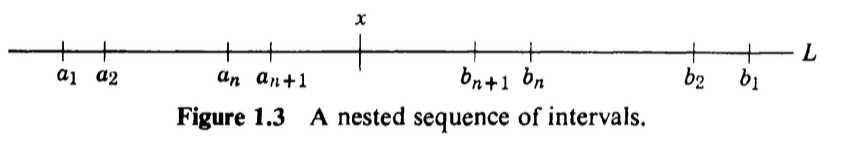
\includegraphics [scale=0.5] {nested_intervals.png} \end{center}
with 
\[ a_1 \le a_2 \le a_3 \le x \le b_3 \le b_2 \le b_1 \]

They say
\begin{quote}let $x$ be confined to a closed interval $I_1 = [a_1,b_1]$ where $a_1$ and $b_1$ are rational.  Within $I_1$ we consider a "subinterval" $I_2 = [a_2,b_2]$ containing $x$, where $a_2$ and $b_2$ are rational.  For example, we may choose for $I_2$ one of the halves of $I_1$, for $x$ must lie in one or both of the halves of $I_1$.  Within $I_2$ we consider a subinterval $I_3 = [a_3,b_3]$ ...  We require that the length of the interval $I_n$ tends to zero with increasing $n$;  that is that the length of $I_n$ is less than any preassigned positive number for all large $n$ ...  A set of closed intervals $I_1, I_2, I_3 \dots$ each containing the next one and such that the lengths tend to zero will be called a "nested sequence of intervals."  The point $x$ is uniquely determined by the nested sequence ... we see that every point $x$, that is, every real number, can be precisely described with the help of infinitely many rational numbers.\end{quote}

\begin{center} 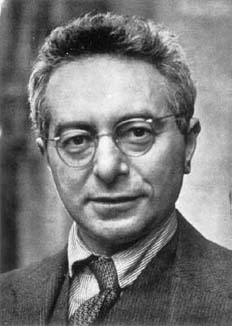
\includegraphics [scale=0.5] {Courant_3.png} \end{center}
Courant

The quote above continues:
\begin{quote}As we shall see, this is an \emph{axiom of continuity}:  it guarantees that no gaps exist on the real axis.  We shall use the axiom to characterize the real continuum and to justify all operations with limits which are basic for calculus and analysis.  (There are also many other ways of formulating this axiom ...)\end{quote}

Compare this description with the process of approximating $\sqrt{2}$ by writing its decimal expansion.

\end{document}